
\chapter{Data-Driven Merchant}
This thesis proposes a merchant software agent that uses demand learning and a dynamic optimization approach to compete with other merchants on online marketplaces.
The merchant makes ordering and pricing decisions with the goal to maximize expected long-term profits.
Demand learning estimates future customer demand from historical customer actions.
The estimated demand is used in a dynamic programming approach to generate optimized ordering and pricing policies.
%what is a policy?

We developed the merchant in four phases to overcome the complexity of this problem.
The first phase in \cref{section:ordering} is constrained to the ordering problem with known customer demand in a monopoly.
Each following phase adds a new difficulty that the merchant must manage.
\cref{section:joint_ordering_pricing} describes the second phase, which adds free choice over the offer price.
The merchant's chosen price will affect sales.
In the third phase (\cref{section:demand_learning}), demand is no longer known and the merchant has to find ways to estimate future demand.
The fourth and last phase (\cref{section:competition}) represents the final problem: The joint ordering and dynamic pricing problem with unknown customer behavior under competition.

\section{Ordering Problem}
\label{section:ordering}
The merchant focuses on the ordering problem in this scenario and makes ordering decisions that promise the most expected long-term profit.
The merchant cannot make pricing decisions, instead all products are sold at a fixed price.
Ordering decisions depend on the customer demand.
The demand is stochastic and its distribution is known to the merchant.
There are no backlogs.
If a customer arrives while the merchant is out of stock, the merchant will miss the sale.
The merchant operates in a monopoly and does not have to care about competitors.

\subsection{Model Description}
\label{subs:ordering_model}
%situation
The merchant sell items over the marketplace.
% price & revenue
Items are offered at a fixed price $a_{fix}$ and each sold item generates the full offer price $a_{fix}$ as revenue.
%discounting
We use discounting to increase the relevance of short-term profits.
A discount factor $\delta$, $0 < \delta \leq 1$, is applied to each time period.
% time horizon
% write about t here?
The time horizon is infinite.
% discrete time %why use discrete time?
The merchant makes exactly one order decision in each discrete time period.

% inventory + holding cost
The merchant holds items in an inventory.
The random inventory level at the start of period $t$ is denoted by $N_t$, ($t = 0, 1, \ldots$).
Storing items in the inventory causes holding costs of $l$ per item per time period, $l > 0$.

%ordering
The merchant can reorder items to increase the inventory level.
The number of items ordered at time $t$ are denoted by $b_t$, with $b_t \geq 0$.
An order of size $b_t = 0$ means that no order is made.
%todo order delay
%set depends on time, yes? no?
The set of admissible orders quantities is denoted $B_t$.
% order cost
Each order causes order costs, which consists of fixed order costs $c_{fix}$ and variable order costs $c_{var}$.
Order decisions influence the merchant's profit based on ordering costs, holding costs, and future potential sales.
%order costs paid upfront
Order costs are defined by:

\begin{equation}
\label{eq:order_cost}
C(b) := \begin{cases}
	c_{fix} + c_{var} \cdot b  & \quad \text{if } b > 0 \\
	0  & \quad \text{if } b = 0
\end{cases}
\end{equation}

%sales
The probability to sell $i$ items within one period of time is denoted by $P(i)$, $(i = 0, 1, \ldots)$.
A changing customer behavior over time is out of scope of this work, thus the sales probability $P(i)$ does not depend on the time period $t$.
The sales probability in the first phase does not directly depend on the price or market situation because the merchant sells at a fixed price in a monopoly.
The random number of sold items within the period $(t-1, t)$ is denoted by $X_t$.
The merchant cannot sell more items than the inventory holds, i.e. $N_t \geq X_{t+1}$, $(t = 0, 1, \ldots)$.

%whats ordering strategy?
%how to write the policy?
Depending on a given ordering policy $(b_t)_t$, the random accumulated discounted profit from time period $t$ is:

$$
G_t := \sum_{s=t+1}^{\infty} (\delta^{s-t} \cdot (a_{fix} \cdot X_s - l \cdot N_{s-1} - C(b_{s-1}(N_{s-1})))
$$

The objective is to find an ordering policy that maximizes the expected total profit $E(G_0 | N_0)$.

% end of model descripiton, maybe write what comes next
%Sales decrease the inventory level over time and orders increase it.

\subsection{Solution Approach}
\label{section:ordering_solution}
%why use dyn prog? -> optimal; why optimal?

%what? -> dyn programming
Goal of this section is to derive optimal ordering policies for the ordering problem.
We use a dynamic programming approach to find the ordering policy promises the best expected profit for the stochastic control problem.
The value function $V_t(n)$ describes the best expected profit $E_t(G_t | N_t)$.
$N_{max}$ denotes an upper limit of the inventory level $n$ and the order decision $b$, $0 \leq n, b \leq N_{max}$. This does not affect the optimal solution as long as $N_{max}$ is greater than the biggest inventory level that can occur in the optimal policy.

%why do we limit time horizon?
We limit the time horizon to the end time $T$.
If $T$ is sufficiently large, the value iteration over $V_t$ converged enough so that the optimal ordering policy is not affected.
The start value $u$ defines the result of the value function at the end of the time horizon, $V_t(n) = u$ for all $n$.
For now, the start value is set to $u := 0$.

%instant vs delayed order, zugangübergänge
We consider $V_t(n)$ with instantaneous and delayed orders.
With instantaneous orders, available items from the start of the time period and the newly ordered items can be sold within that period.
The following time period starts with an inventory of items that were not sold in the previous period.
With delayed orders, only items that are available from the start of the time period can be sold within that period.
The following time period starts with an inventory of items that were not sold in the previous period plus the number of items ordered in the previous period.

The value function with an instantaneous arrival of orders is:
%todo special case P(n_max) -> rest probability
\begin{equation}
\begin{split}
V_t(n) = \max_{b \in B_t} \Bigg\{
\sum_{i = 0}^{N_{max}}
P(i) \cdot \Big(
(a_{fix} \cdot min(i, n + b) %sales
- l \cdot (n + b) % holding cost
- C(b)) % order cost
 \\
+ \delta \cdot V_{t+1}\big(min(max(n + b - i, 0), N_{max}))\big)
\Big)\Bigg\}
\end{split}
\label{eq:dyn_prog_no_delay}
\end{equation}

%todo: order delay mentioned in model description?
The value function with order delay is shown in the following equation:

\begin{equation}
\begin{split}
V_t(n) = \max_{b \in B_t} \Bigg\{
	\sum_{i = 0}^{N_{max}} 
		P(i) \cdot \Big((
			a_{fix} \cdot min(i, n) %sales
			- l \cdot n % holding cost
			- C(b) % order cost
		) \\
		+ \delta \cdot V_{t+1}\big(min(max(n - i, 0) + b, N_{max}))\big)
	\Big)\Bigg\}
\end{split}
\label{eq:dyn_prog}
\end{equation}

The set of order quantities $B_t$ is a discrete set of integers and must contain zero to allow the merchant to make no order.
The optimal ordering decision $b^*(n)$ is given by using arg max on \cref{eq:dyn_prog_no_delay,eq:dyn_prog}.

That is for instantaneous orders

\begin{equation}
\begin{split}
b^*(n) = \argmax_{b \in B_t} \Bigg\{
\sum_{i = 0}^{N_{max}}
P(i) \cdot \Big(
(a_{fix} \cdot min(i, n + b) %sales
- l \cdot (n + b) % holding cost
- C(b)) % order cost
\\
+ \delta \cdot V_{1}\big(min(max(n + b - i, 0), N_{max}))\big)
\Big)\Bigg\}
\end{split}
\end{equation}

and for delayed orders

\begin{equation}
\begin{split}
b^*(n) = \argmax_{b \in B_t} \Bigg\{
\sum_{i = 0}^{N_{max}} 
P(i) \cdot \Big((
a_{fix} \cdot min(i, n) %sales
- l \cdot n % holding cost
- C(b) % order cost
) \\
+ \delta \cdot V_{1}\big(min(max(n - i, 0) + b, N_{max}))\big)
\Big)\Bigg\}
\end{split}
\label{eq:optimal_order}
\end{equation}

Equation \cref{eq:optimal_order} is the optimal solution to the ordering problem if the order delay is exactly the length of a time period.
It is possible to find optimal ordering policies for arbitrary order delays using this dynamic programming approach.
However, this greatly increases the dynamic programming state and results in long computation times.
In order have reasonable decision times for the merchant, we use the presented approach, which is a heuristic for order delays different from the length of the time period and otherwise an exact solution.
The following phases will only consider the variation with delayed orders.

\subsection{Evaluation}

\subsubsection{Numeric Example}
\todo{show solution for specific parameters, compare policy with/without delay}
%compare effect of parameter on policy

\subsubsection{Effect of Start Value $u$ on $V_0(n)$}
In \cref{section:ordering_solution}, we used an arbitrary start value $u := 0$ and claimed that the value function $V_0(n)$ converges to the optimal expected profit if $T$ is sufficiently large.
In the following example we show that the value function converges to the same value independently from the start value.

\cref{fig:convergence} shows results of $V_0(0)$ with varying $T$ and start values $V_T$.
The value function converges to the same result for any $V_T$.
It does not matter if the start value is bigger or smaller than the resulting expected profit.
However, the value function converges earlier if $V_T$ is near the optimal expected profit.
%direct ref to section?
We will use this fact in later sections to speed up the policy computation.

\begin{figure}[t]
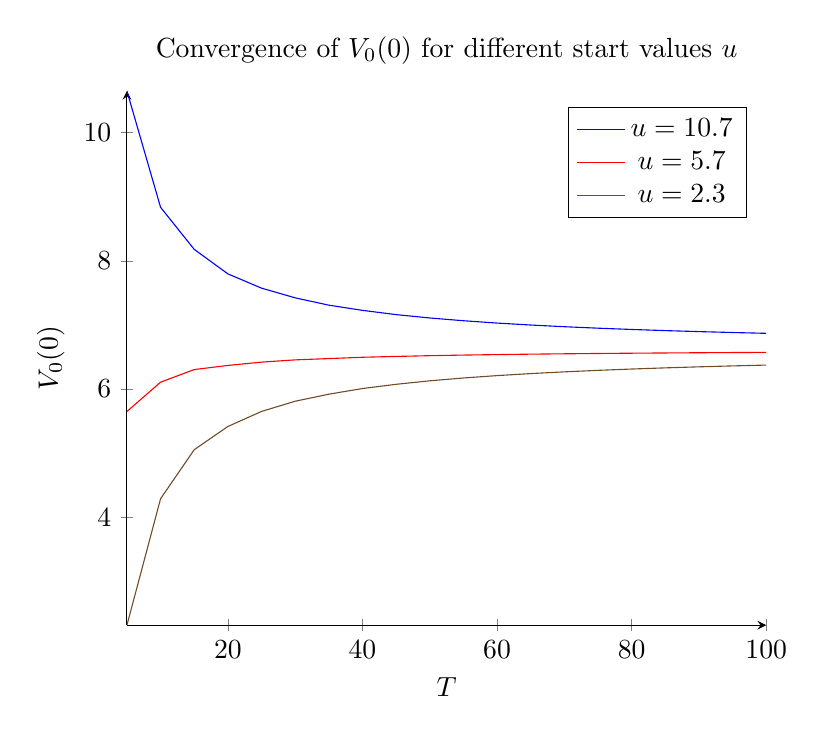
\begin{tikzpicture}
\begin{axis}[
title={Convergence of $V_0(0)$ for different start values $u$},
xlabel={$T$},
ylabel={$V_0(0)$},
legend pos=north east,
grid style=dashed,
axis lines = left,
width=0.8\textwidth,
]

\addplot+[mark=none]
coordinates {(5, 10.650190245476479)(10, 8.8349323075140394)(15, 8.1792648210654963)(20, 7.7971329777749263)(25, 7.5742589181038458) (30, 7.4232242422163681)(35, 7.308928579872326)(40, 7.2279708622948116)(45, 7.161335085202075)(50, 7.1089572918512074) (55, 7.0660029726563431)(60, 7.0295402644629057) (65, 6.9991371516213245) (70, 6.9726912293655996) (75, 6.9498393709566395) (80, 6.929825937583602) (85, 6.9120734346116484) (90, 6.8963337508543576) (95, 6.8821968575926808) (100, 6.8694716786018226)};
\addlegendentry{$u = 10.7$}

\addplot+[mark=none]
coordinates {(5, 5.6501902454764794) (10, 6.1076595802413101) (15, 6.3042648210654928) (20, 6.3685615492034966) (25, 6.4204127642576871) (30, 6.4554823067324927) (35, 6.4755952465389939) (40, 6.4962635452216384) (45, 6.5091611721585938) (50, 6.5207219977335571) (55, 6.5302886869420531) (60, 6.5377369857743801) (65, 6.5445916970758642) (70, 6.550156018097991) (75, 6.5551025288513722) (80, 6.5594555672132291) (85, 6.5632362253093195) (90, 6.5666634211840238) (95, 6.5696968575926782) (100, 6.5724419756315244)
};
\addlegendentry{$u = 5.7$}

\addplot +[mark=none]
coordinates {
	(5, 2.3168569121431455) (10, 4.2894777620594917) (15, 5.0542648210654928) (20, 5.4161805968225405) (25, 5.651181995026918) (30, 5.8103210164099108) (35, 5.9200396909834385) (40, 6.0084586671728593) (45, 6.0743785634629441) (50, 6.1285651349884596) (55, 6.1731458297991981) (60, 6.2098681333153616) (65, 6.2415613940455641) (70, 6.2684658772529209) (75, 6.2919446341145315) (80, 6.3125419869663153) (85, 6.3306780857744362) (90, 6.3468832014038048) (95, 6.3613635242593451) (100, 6.3744221736513262)};
\addlegendentry{$u = 2.3$}

\end{axis}
\end{tikzpicture}
\caption{This chart shows how the start value $u$ influences the final expected profit $V_0$. The function converges with any start value to the same expected profit, given a sufficiently large $T$. However, $V_0$ converges earlier if $u$ is near the optimal expected profit.}
\label{fig:convergence}
\end{figure}

%told, that this is a optimal ordering policy
%deviations from that should result in worse performance (profit)
%let's compare computed optimal policy in monopoly with policy that orders one item more(less)
%hint: use bigger dif if you cannot see difference in policies
\todo{compare different n}

\section{Joint Ordering and Pricing}
\label{section:joint_ordering_pricing}
%What?
In this section, the merchant is in the same situation as in \cref{section:ordering} but additionally gains control over the selling price.
With ordering and pricing decisions enabled, the merchant's actions on the marketplace are unconstrained.
%Difference in demand
Demand in this scenario depends on the chosen selling price.
A higher price typically results in less demand.
As in the previous problem, the demand distribution is known.

%Why joint:
We cannot separate the inventory and pricing problem and solve each in isolation to solve the whole problem optimally.
Ordering and pricing decisions influence each other.
Setting a price changes the demand, which requires a different ordering policy.
The other way around, an ordering policy might require certain prices for a better control over inventory levels.
This mutual influence is the reason, why ordering and pricing should be decided jointly.
However, this is a more complex problem compared to solving the ordering problem and pricing problem separately.

\subsection{Model Description}
\label{subs:joint_model}
This model is an extension of the model from \cref{subs:ordering_model}.
%pricing decision
Instead of a fixed selling price $a_{fix}$, the merchant sets a price $a_t$ in each period $t$, with $a_t \geq 0$.
The set of admissible pricing decisions is denoted $A_t$.
%revenue
Each sold item in period $t$ generates a revenue of $a_t$.

%demand
The probability to sell $i$ items depends now on price $a$.
The merchant knows the price-dependent probability distribution in this scenario.

Depending on a given pricing and ordering policy $(a_t, b_t)_t$, which can depend on the current inventory level, the random accumulated discounted profit from time period $t$ is:

$$
G_t := \sum_{s=t+1}^{\infty} (\delta^{s-t} \cdot (a_{s-1}(N_{s-1}) \cdot X_s - l \cdot N_{s-1} - C(b_{s-1}(N_{s-1})))
$$

The objective is to find a joint pricing and ordering policy that maximizes the expected total profit $E(G_0 | N_0)$.

\subsection{Solution Approach}
\label{section:joint_solution}
As a basis, we use the dynamic programming approach shown in \cref{eq:dyn_prog}.
The action space is extended by one dimension that contains all potential pricing decisions $A_t$.

%todo remove t from A and B.
\begin{equation}
\begin{split}
V_t(n) = \max_{\substack{b \in B_t \\ a \in A_t}} \Bigg\{
\sum_{i = 0}^{N_{max}}
P(i, a) \cdot \Big((
a \cdot min(i, n) %sales
- l \cdot n % holding cost
- C(b) % order cost
) \\
+ \delta \cdot V_{t+1}\big(min(max(n - i, 0) + b, N_{max}))\big)
\Big)\Bigg\}
\end{split}
\label{eq:dyn_prog_joint}
\end{equation}

There are three changes to the value function.
The probability is price-dependent ($P(i, a)$), the revenue in one period depends on the chosen price ($a \cdot min(i, n)$), and the action space is extended by the set of pricing decisions $A_t$.
The optimal ordering policy $b^*_t(n)$ and pricing policy $a^*_t(n)$ are given by

\begin{equation}
\begin{split}
(a^*_t(n), b^*_t(n)) = \argmax_{\substack{b \in B_t \\ a \in A_t}} \Bigg\{
\sum_{i = 0}^{N_{max}}
P(i, a) \cdot \Big((
a \cdot min(i, n) %sales
- l \cdot n % holding cost
- C(b) % order cost
) \\
+ \delta \cdot V_{1}\big(min(max(n - i, 0) + b, N_{max}))\big)
\Big)\Bigg\}
\end{split}
\label{eq:joint_best_price_order}
\end{equation}

%todo schreibe hier irgendwas hin, nicht mit gleichungen enden

\subsection{Evaluation}
\todo{numeric example; show policies with increasing prices}
% anything else I can show here?
% compare different parameters, effect on price or on order
\section{Demand Learning}
\label{section:demand_learning}

This section extends the joint inventory and dynamic pricing problem from \cref{section:joint_ordering_pricing} by not providing the merchant with sales probabilities.
%the merchant, the merchant, the merchant...
The merchant needs to estimate the customer behavior in order to make effective ordering and pricing decisions.
The merchant can get information about the customer behavior from past customer actions.
The merchant can analyze historical market situation and sales in order to deduce future sales probabilities.
%what is this dat, where is it from? (how does it look like?)
This is called demand learning.

%from data to demand distribution

%model section removed, maybe mention somewhere that problem is same, only prob is not know

\subsection{Solution Approach}
In order to overcome the inventory and dynamic pricing problem with missing demand information, we split the whole problem into two parts.
The first part is the training of a model from historical market situations and sales in order to predict sales probabilities.
These probabilities are used in the second part to create optimized ordering and pricing policies.
%why sales prob = demand prob? check whole section
Given predicted sales probabilities, the dynamic programming solution from \cref{section:joint_solution} can be used as it is, to calculate ordering and pricing policies.

Assuming, the merchant predicts sales probabilities correctly, the dynamic programming approach creates optimal policies.
In other cases, the quality of policies will depend on the accuracy of predictions. 
The separation of demand prediction and policy creation lets us focus on the prediction of the demand probabilities, while having a working solution for the policy creation.

%bring data into right form
In order to use market and sales data for demand learning, it must be transformed into a usable form.
From the market data we know, at what times the market situation changed and what the market situation was.
The sales data contains information about all of a merchant's sales, including when the sales happened.
These two data sources can be combined and aggregated to a form that contains the number of sales per time period for each market situation.
The size of a period corresponds the period in which the merchant makes a order and pricing decision.

%bring data into right form, part 2 feature extraction
We use regression analysis for the demand learning.
Regression analysis models and analyzes the relationship between a dependent variable and explanatory variables.
In this case, the dependent variable is the sales per period metric.
Independent variables are extracted from the market situation.
In this scenario, the demand depends only on the merchant's price.
%motivation: why use linear regression and not something else? is relationship linear?
We use linear regression to find a relationship between the explanatory variables $\vec{x}(\vec{s})$ of a market situation $\vec{s}$ and the sales per period for this situation.
The following equation shows how to predict mean sales per period for a market situation $\vec{s}$.

\begin{equation}
\label{eq:linear_regression}
\lambda(\vec{s}; \vec{\beta}) = \vec{x}(\vec{s})^\intercal \cdot \vec{\beta}
\end{equation}

$\vec{\beta}$ are the weights of the regression model.
Given observed sales per period $y_1, y_2, \ldots, y_J$ and explanatory variables $\vec{x}_1, \vec{x}_2, \ldots, \vec{x}_J$ from $J$ historical market situations, the optimal weights $\vec{\beta}^*$ are calculated with the linear least squares objective:

\begin{equation}
\vec{\beta}^* = \bigg(\sum_{i=1}^J{\vec{x}_i \vec{x}_i^\intercal} \bigg)^{-1}
			  \bigg(\sum_{i=1}^J{y_i \vec{x}_i} \bigg)
\end{equation}

%predicted mean demand -> distribution
The merchant is able to predict mean sales per period for a market situation with the regression analysis.
However, sales probabilities are needed for the dynamic programming approach.
The mean sales per period can be used as a parameter to create a suitable probability distribution.
%find better citation with a study or something to show that.
We describe the demand distribution with a Poisson distribution.
This discrete distribution is a good approximation for the arrival and buying process of customers \cite{DBLP:journals/ior/Wolff82}.
Equation \ref{eq:probability} shows the calibration of the Poisson distribution with the linear regression from \cref{eq:linear_regression} in order to obtain estimated sales probabilities for a market situation $\vec{s}$.

\begin{equation}
\label{eq:probability}
P(i, \vec{x}) :=
	e^{-\lambda(\vec{s}; \vec{\beta}^*)}
	\frac{\lambda(\vec{s}; \vec{\beta}^*)^{i}}{i!}
\end{equation}

This sales probability function is used in \cref{eq:joint_best_price_order} to calculate optimal ordering and pricing policies.

%retraining
The merchant has access to a steadily growing collection of market situations and sales data over time.
The quality of predictions is increased by periodic trainings that utilize the new data.
There is no sales data available at the start of a merchant's career on the online marketplace.
In that case, we use a rule-based ordering and pricing strategy until enough training data is available.
The rule-based pricing strategy sets random prices to explore the customer behavior in different market situations.
The exploration pricing strategy sets random prices.
This allows the merchant to encounter many different market situations and obtain sales data for these situations.

%features + algo
%gebe ich constant an?
Our explanatory variables $\vec{x}$ consists of the price $p$ and the constant 1.
Other variations like $\sqrt{p}$ or $p^2$ are possible to recognize non-linear relations to the price.
$\vec{x}$ will be extended by additional variables in the next phase.
Additionally, the linear regression algorithm can be easily replaced by another regression approach like decision tree regression.

\subsection{Evaluation}

\todo{show how good predicted percent to real percent is}


\todo{show prediction quality over number of training examples}

\section{Competition}
\label{section:competition}
Until now, the merchant offered items on the marketplace in a monopoly.
This is usually not the case on real online marketplaces.
Other merchants offer the same or similar products and everyone competes for market share.
A common strategy to do that is to offer the cheapest price.
When multiple merchants pursue this strategy, the price will spiral downwards.
Such a commercial competition is called price war.
It is not the best strategy to always undercut the competitors because of decreasing profit margins.
Sometimes it is better to also raise prices.
This reduces sales, but the profit margin is higher.
This section proposes a merchant that makes optimized ordering and pricing decisions under competition with the goal to maximize profit.

In the previous sections, the sales probability was only influenced by the merchant's own pricing decisions.
In this scenario, the merchant's sales probability is also influenced by competitor's offers.
%model description
The model is the same as in \cref{subs:joint_model} with the exception that the number of sold items $X_t$ within a period depends on the merchant's offer price and the competitor's offer prices.
Merchants have access to historical market and sales data.
The market data contains competitors' prices.
However, sales data is limited to the merchant's own sales and does not contain sales from competitors.

%merchant must be fast
Market situations can change frequently on online marketplaces.
A merchant must be able to quickly and effectively react on new market situations in order to offer an suitable price for the new situation.
Getting fast decisions is a challenge because the increasing complexity of the inventory and dynamic pricing problem over the last sections resulting in solutions with increasing computational effort.
Nevertheless, there are ways to improve the speed of the dynamic programming approach which are described in \cref{section:faster_dyn_prog}.

\subsection{Solution Approach}


%build on top of solution from previous section


%describe two possible approaches
%todo reread, and split paragraph
The inventory level was the only state on which ordering and pricing decisions were based on in the previous problems.
With competitors on the marketplace, the merchant must also consider their offers when making ordering and pricing decisions.
One possible approach is to add competitors' offers to the state in the dynamic programming calculation.
We decided against this solution because it drastically increases the state by multiple dimensions and therefore slows the computation down by multiple orders of magnitude due to the curse if dimensionality.
Moreover, demand learning must predict transitions of competitors' offers from one time period to another.
This means that competitors' strategies must be learned, which requires a substantial amount of trainings data and a complex demand model to make sensible predictions.
Instead, we take the following approach.
We create ordering and pricing policies whenever the market situation changes for that specific new market situation.
The ordering and pricing decisions for this approach depend only on the merchant's inventory level.
This keeps the computation fast and efficient.
Additionally, only sales probabilities are predicted but not the competitors' price reactions.
This can be done by a relatively simple demand model, which can make good predictions even with few market and sales data.
The disadvantage is that new policies must be computed for each new market situation.
The next sections tackles the problem of how to quickly compute ordering and pricing policies for new market situations.

%market situation more complex -> more features
Market situations become more complex with the introduction of competition.
Previously, there was at most one active offer at a time.
In this scenario, a market situation can contain as many offers as there are participating merchants.
And the number of offers can change over time when merchants are out of stock.
In \cref{section:demand_learning}, the merchant's offer price was sufficient to describe a market situation.
With competition, the sales probability of an offer depends not only on its price but also on the price of the other offers.
New explanatory variables are necessary for demand learning to describe the more complex market situations.
We created two new explanatory variables besides the offer price in order to describe market situations with competition.
The variables are explained in detail below.

\begin{description}
	\item [Own price]
		This explanatory variable hold the value of the merchant's current offer price.
		It helps to explain effects on the sales probability that are based on the total price.
		For example, a higher price generally results in less demand.
	\item [Price rank]
		This variable describes the merchant's relative position in the price ranking.
		The price rank is defined by the number of competitors' offer that cost equal or less than the merchant's offer.
		Demand learning uses this to find a relationship to the sales probability.
		For example, it is probable that a merchant sells more items by having the cheapest offer instead of the second cheapest.
	\item [Price difference to cheapest offer]
		This is the difference in price from the merchant's offer to the cheapest offer.
		If the merchant has the cheapest offer, the variables value will be €0.
		It is a relative variation of the 'own price' metric.
		This variable could explain effects like: a customer is willing to pay €5 more than the cheapest product but not €10 more.
\end{description}

With these explanatory variables it is possible to describe the effect of the competition and the merchant's offer price on the sales probabilities.

The predicted sales probability are used in the dynamic programming approach to compute ordering and pricing policy.
As explained above, the policies are computed for each new market situation.
At this point, the computation takes around 10 seconds to complete.
This is to long for the merchant to quickly and frequently react on the changing market.
In the next section, we will reduce this time to allow shorter decision intervals for the merchant.

%todo dyn progamming formula with p(i,x) in demand section
%todo make x depend on price somehow

\subsection{Efficient Dynamic Programming}
\label{section:faster_dyn_prog}
In this section, we present four approaches to increase the computational efficiency of dynamic programming.
These approaches are applied to our merchant to reduce time spent on computing policies.
This allows the merchant to react faster on new market situations.
The approaches are: using a better start value, adapt decision sets, and tweaking the number of iterations.

%better start value
%check: mache abschnitt verständlicher
\cref{fig:convergence} shows that dynamic programming converges faster if the start value $u$ is near the final expected profit.
We assume that the expected profit from two successive market situations is similar because the market situations will not fundamentally change in that short time frame.
Setting the $u$ to the expected profit from the previous computation will reduce the time until dynamic programming converges.
Even if the assumption does not hold true and there is a big change in expected profit, the computation converges most of the time faster than with our previous start value $u = 0$.

%adapt decision sets
%todo remove t from decision set A and B
%very passiv part
Another way to increase the efficiency of the dynamic programming approach is to change the set of pricing decisions $A$ and set of ordering decisions $B$ to only contain relevant decisions.
E.g., a order quantity of 100 is an irrelevant decision if the final policy only uses order quantities around 10.
The irrelevant decision can be removed from the decision set without affecting the result.
%better name/include for T
The dynamic programming approach is run for a reduced number of periods $T$ for approximations of pricing and ordering policies.
%maybe explain this with min, max
After that, new decision sets are created, containing the range of decisions that occur in the approximated policy.
The ranges are increased by some constant to contain decisions that were not used before.
The new decision sets are used to compute pricing and ordering policies again.
The second dynamic programming computation is faster because it works on a reduced pricing and ordering decision sets.
This process can be repeated in order to adapt the decision sets multiple times.
This approach is not only faster than computing policies on the full decision sets, it also removes the limitation of having a static lower and upper limit on the price and order quantity.
The decision sets can be adapted until they contain relevant decision.
No prior knowledge of relevant prices and order quantities is necessary.
%mention 0 special value for order decisions?
%stop after x iterations or until policy converged
%quantisation (not done here) (range vs stride)

%change number of iteration
The end time $T$ is a parameter that affects the number of iterations and therefore the computation time of the dynamic programming approach.
The choice of this parameter is a trade-off between precision for large $T$ and efficiency for small $T$.
One observation is that the policy converges faster than the calculated expected profit.
This can be used to reduce $T$ without affecting the precision of the resulting policies.
It is possible to further reduce the end time $T$, if approximations of the optimal pricing and ordering policies are sufficient.

%show speed increase, maybe here maybe in eval

\subsection{Evaluation}
%todo need some intro text here

\subsubsection{Efficient Dynamic Programming}
%check: have i mentioned early stopping in text?

The goal of our efficient dynamic programming approaches is to reduce the computation time in order to be able to react faster to new market situations.
We measured the runtime performance of the dynamic programming variations to show the impact of the optimizations.
All variations calculate pricing and ordering policies for the same market situation for a comparison.
The market situation contains one own offer and two competitor offers.


%baseline
The baseline for the measurements is the pure dynamic programming approach without any of the methods from \cref{section:faster_dyn_prog}.
We set the end time $T = 500$, i.e., 500 iterations.
%use last value (why faster -> less iterations)
The first optimization method sets the start value $V_T$ to the expected profit from the last computation.
This way $V_T$ is closer to the final expected profit compared to $V_T = 0$.
The value function converges earlier with an appropriate start value.
We utilize this fact and reduce the number of iterations to 200 in order to decrease the computation time with only a minimal precision loss.
%adapt decisions (also reuses space)
The next optimization method is the adaption of the ordering and pricing decision sets.
We makes 5 successive dynamic programming calculations with 40 iterations each.
This are in total again 200 iterations, but the decision sets are adapted between calculations.
This reduces the size of the decision sets without omitting relevant decisions.
Relevant decisions are decisions that occur in the optimal policy.
Smaller decisions sets lead to a more efficient computation of pricing and ordering policies.
Adapted ordering and pricing decision sets are reused from the previous computation similarly to the start value.
%early stopping
The last optimization method is early stopping.
This stops the dynamic programming calculation if the ordering and pricing policies do not change after a number of iterations.
The assumption is that the polices are already converged, or are almost converged and are close enough to the optimal policy.
Early stopping saves computation time by cutting out iterations that do not have a great impact on the resulting policies.
The results are listed in \cref{tab:speedup}.
Note that each row in the table also contains the optimizations from the rows above.

\begin{table}[t]
	\centering
	\begin{tabular}{ lrr }
		\toprule
		Optimization Method & Computation Time [ms] & Error [\%] \\
		\midrule
		Baseline & 9425 & 0.53 \\
		\makecell[l]{Set start value to \\ result of previous computation} & 3734 & 0.98 \\
		Adapt ordering \& pricing decisions & 1550 & 5.71 \\
		Early stopping & 747 & 5.71\\
		\bottomrule
	\end{tabular}
	\caption{These are the results of the computation time optimizations applied to the dynamic programming approach.
	Each row contains a new optimization method and the methods from the rows above. The last column shows the difference between calculated and actual expected profit of 18.68.}
	\label{tab:speedup}
%calculated expected profits
%18.5891472589
%18.5045225348
%16.5739895402
%16.5740436621
% actual:
%18.6885701077
\end{table}

Applying all three optimization methods to the dynamic programming approach reduces the computation time in our example from 9.4 seconds to 0.75.
This is fast enough to quickly update prices after a new market situation.
These optimizations come at the cost of precision of the dynamic programming approach.
The precision loss for setting the start value to the expected profit from the previous result and for early stopping are neglectable.
In contrast, the adaption of the decision sets introduce an error of around 5\% to the resulting expected profit.
Despite the precision error, the computed policies usually are identically to the optimal policy.
We are willing to accept the the loss in precision in order to increase the efficiency of the dynamic programming approach.

\subsubsection{Oligopoly Simulation}
This section shows how our merchants performs in an oligopoly.
The merchants sell products on the \pricewars platform.
The objective is to maximize the profit.

\begin{figure}[p]
	\centering
	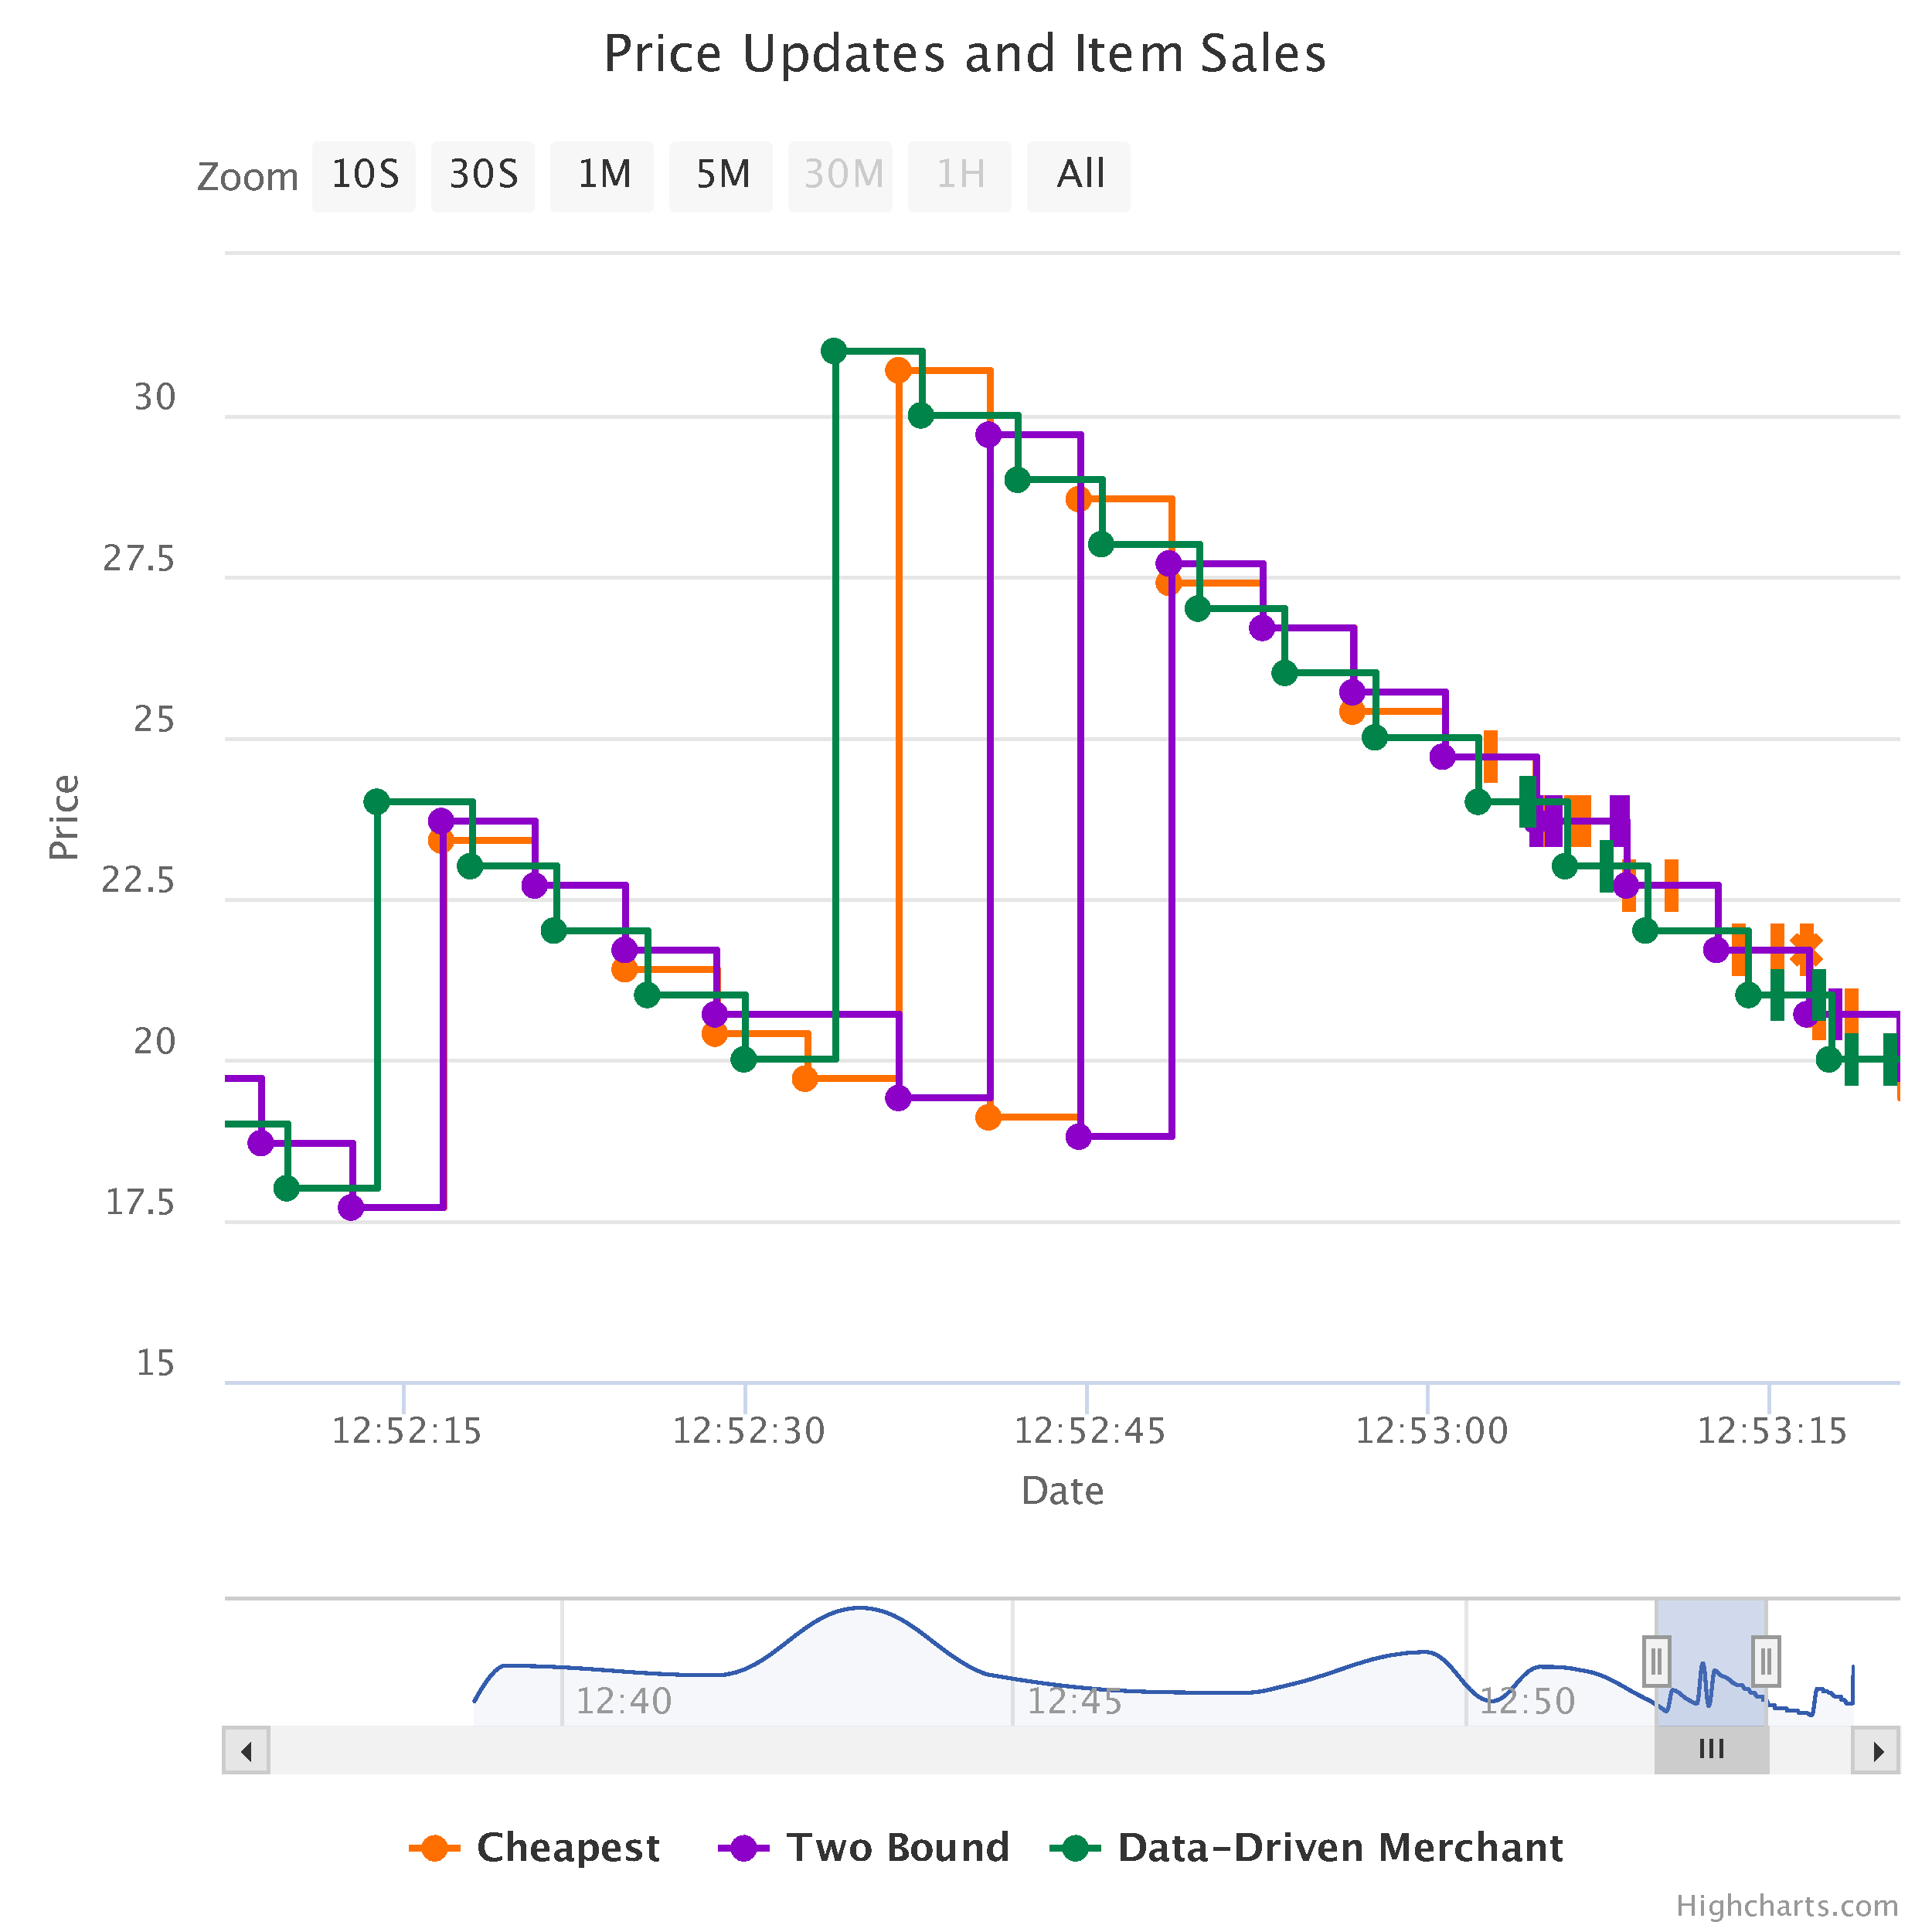
\includegraphics[width=0.8\textwidth]{figures/competition_prices.pdf}
	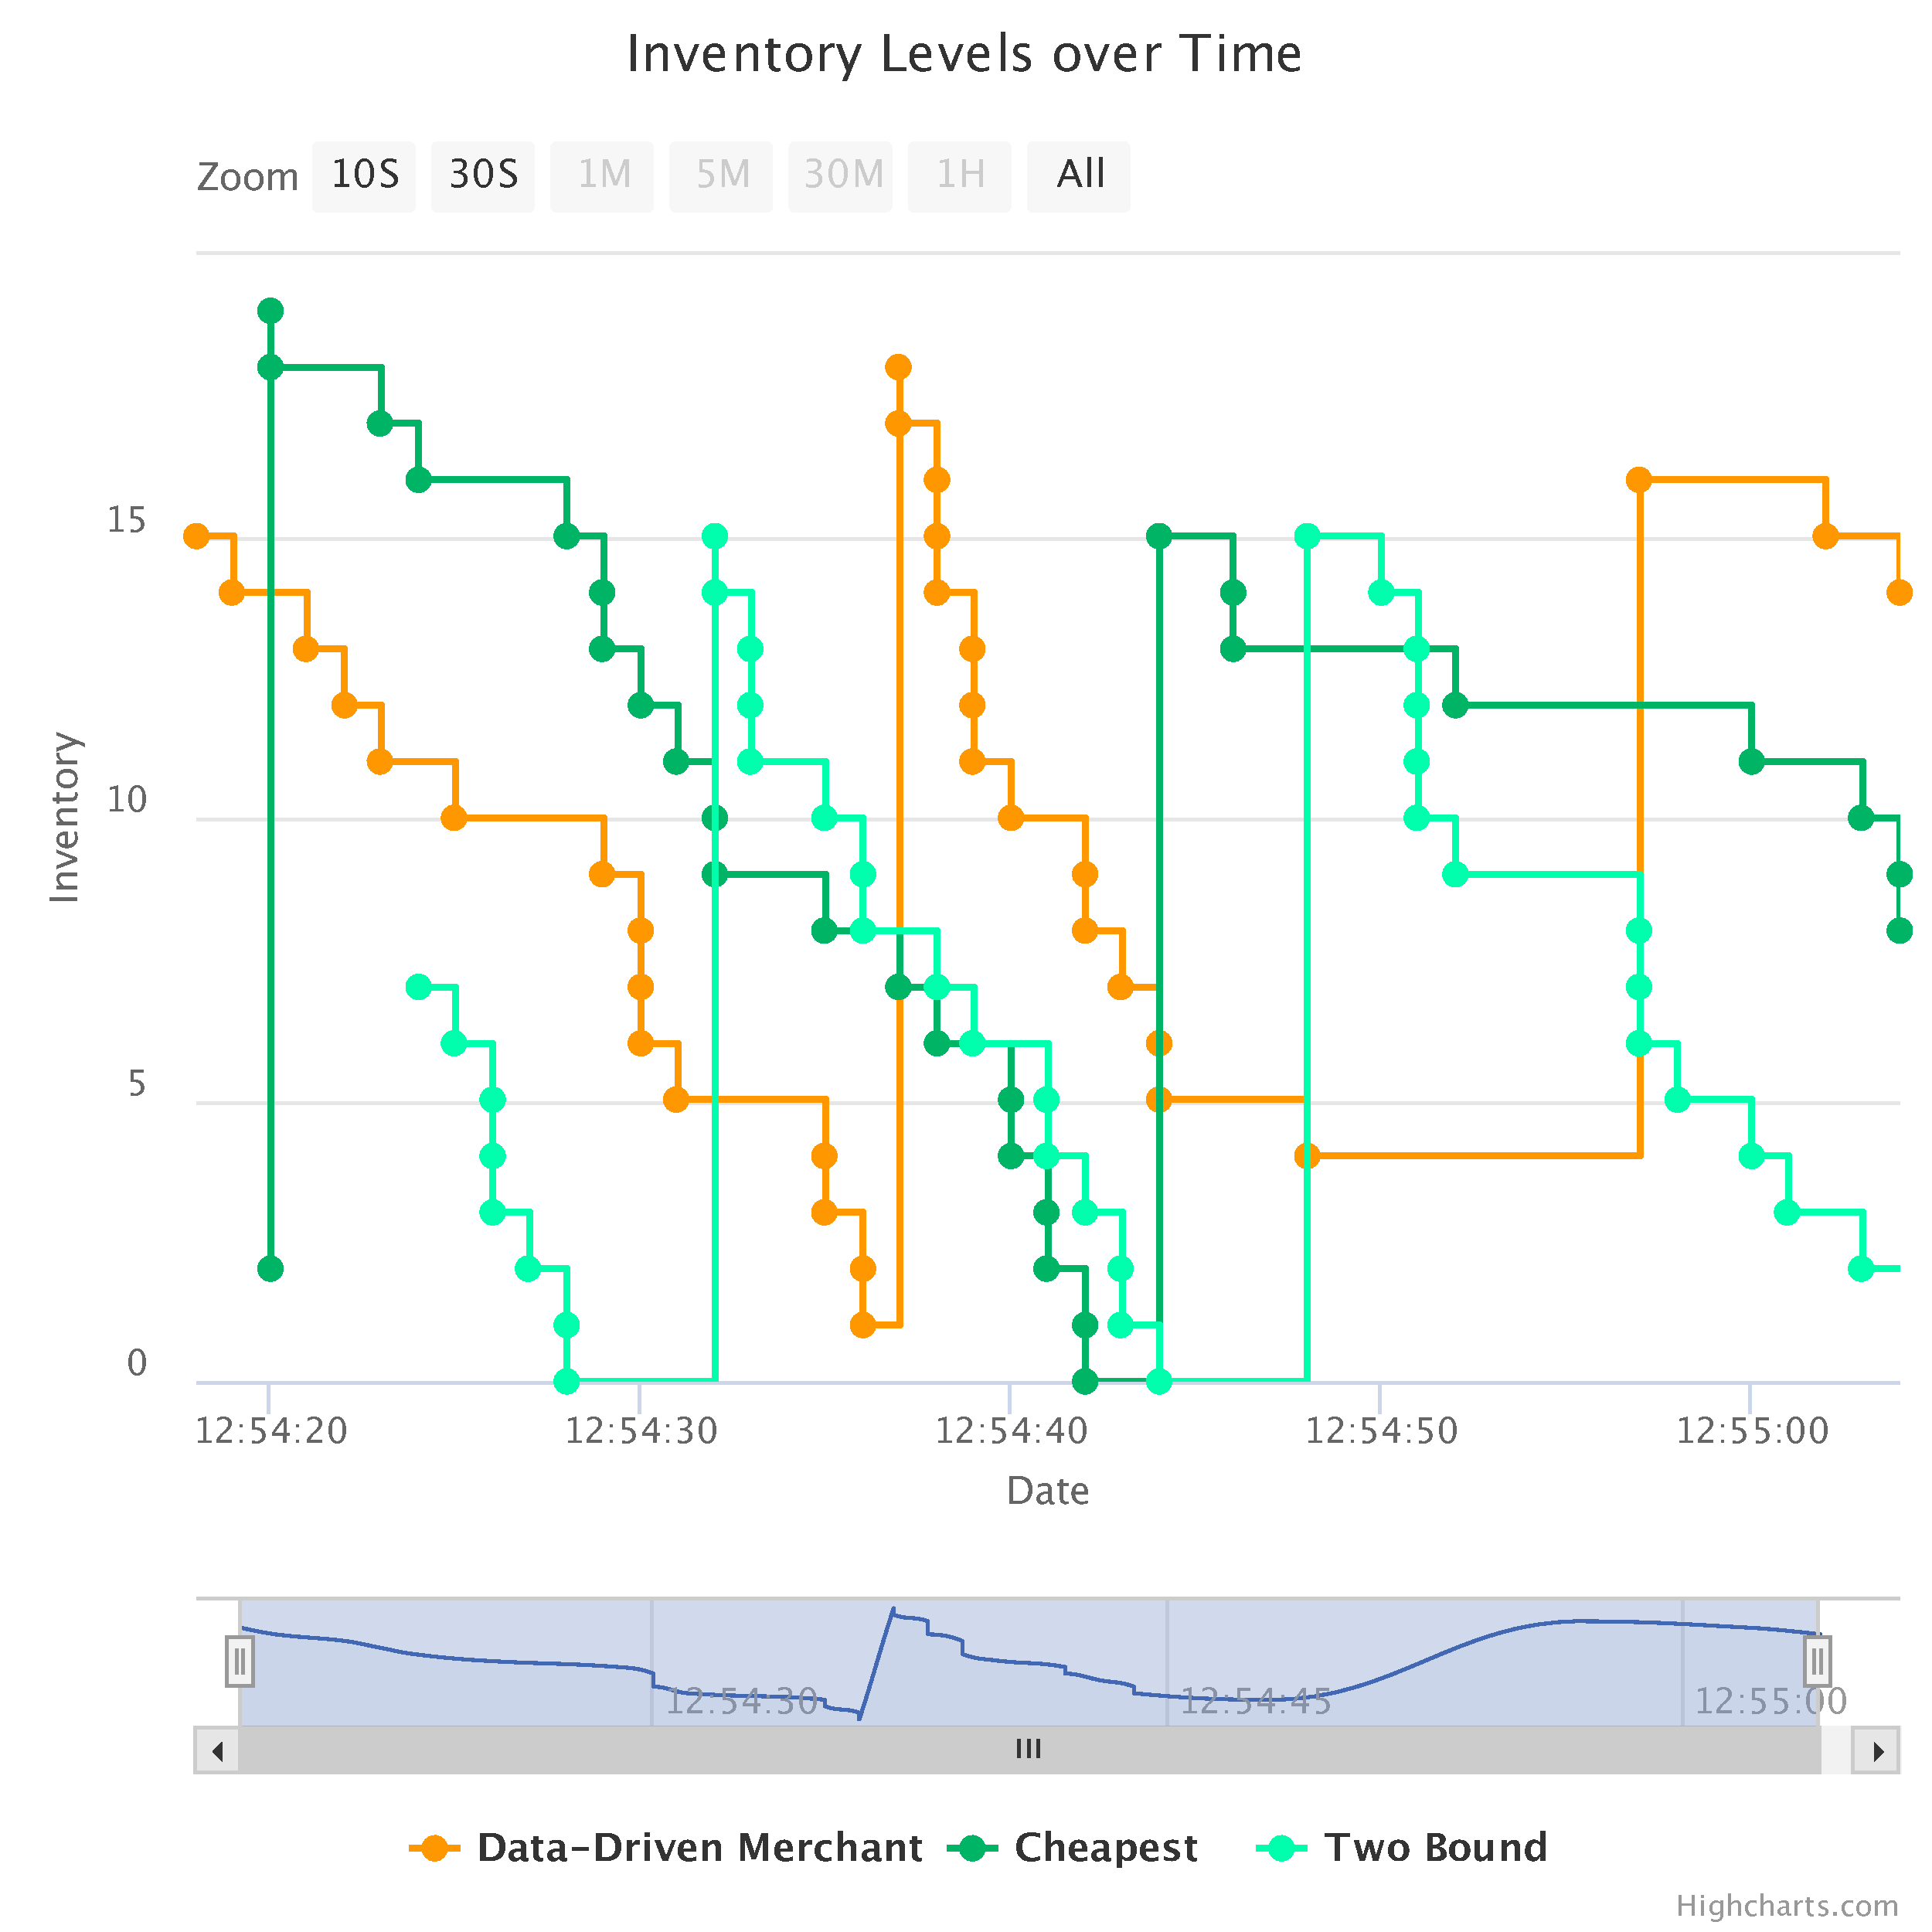
\includegraphics[width=0.8\textwidth]{figures/competition_inventory.pdf}
	\caption{Price trajectories and inventory levels over time from an oligopoly scenario on the \pricewars platform. Our data-driven merchant competes with two rule-based merchants.}
	%analyze bahavior in one sentence?
	\label{fig:competition}
\end{figure}

%present rule-based merchants
Our merchant, called data-driven merchant, competes with two rule-based merchants.
The cheapest merchant always undercuts competitors in order to offer the cheapest product.
%check: but as high to be still cheapest
The cheapest merchant tries to have the most sales by offering the best price.
This merchant does not have a lower price limit and is willing to undercut competitors down to €0.
The second rule-based merchant, called two bound merchant, undercuts competitors similarly to the cheapest merchant.
However, the merchant has a upper and lower price bound.
If offer prices go below the lower price bound, the two bound merchant raises prices to the upper bound.
Moreover, the upper price bound is the maximum price that this merchant will set.
Both rule-based merchants have a static ordering policy.
They order whenever the inventory level falls below a threshold and order as many items to reach a certain inventory level.

We simulated the scenario with competition on the \pricewars platform.
The management UI shows pricing and ordering decisions during the simulation (see \cref{fig:competition}).
The data-driven merchant learned the advantage of undercutting competitors' offers.
However, this creates a price war and offer prices decrease.
With shrinking profit margins, it becomes unprofitable to set the price below competitors' prices.
The data-driven merchant pushes the price up in such a situation.
This action is especially successful if the competitors also increase their offer prices.

\begin{table}[t]
	\centering
	\begin{tabular}{lrrrr}
		\toprule
		Merchant & Profit & Revenue & Holding Cost & Order Cost \\
		\midrule
		Data-Driven & 5944.13 & 21938.00 & 943.87 & 15050.00 \\
		Cheapest & 5386.90 & 23770.80 & 903.89 & 17480.00 \\
		Two Bound & 5038.63 & 20148.30 & 644.67 & 14465.00 \\
		\bottomrule
	\end{tabular}
	\caption{Simulation results of the oligopoly scenario. The data-driven merchant made the most profit. The cheapest merchant made the most revenue.}
	\label{tab:competition}
\end{table}

\cref{tab:competition} shows the results of a half an hour competition between three merchants.
The data-driven merchant outperformed all competitors.
Our data-driven merchant made around 10\% more profit than the cheapest merchant and 18\% more than the two bound merchant.
Interestingly, our merchant did not make the most revenue, but the cheapest merchant did.
The cheapest merchant sold the most items but with low profit per item.
Our merchant made the most profit by saving a lot of order cost compared the to cheapest merchant.
The data-driven merchant orders on average more items than the competitors.
This results in higher holding costs but saves on fixed order cost.

%command: python3 helper_scripts/benchmark.py -o ../runs -d 30 --merchants "python3 /home/carsten/pricewars-merchant/merchant.py --port 5000 --strategy Cheapest" "python3 /home/carsten/pricewars-merchant/merchant.py --port 5001 --strategy \"Two Bound\"" "python3 /home/carsten/pricewars-merchant/merchant_scenario4.py --port 5002" --holding_cost 3

\todo{show reaction when changing demand or fixed ordering cost}
%

\section{Implementation}
%todo ref python and libs
%how is merchant implemented? (language choice)
Merchants on the \pricewars platform can be written in any language as long as they comply with the platform's REST APIs.
%ref to pytho
We decided to implement our merchant in the Python programming language for the following reasons.
Python has great library support for numerical computing.
These libraries allow a concise and efficient implementation without reinventing the wheel.
The \pricewars platform offers a library written in Python, that implements the APIs to communicate with the platform's services.
Lastly, it is possible to quickly create prototypes in that language.

%architecture
Our merchant consists of four components as it is shown in \cref{fig:merchant_architecture}.
%motivation for this architacture
%main loop
The main loop is the central component.
It regularly checks the marketplace for open offers, updates prices, and orders items from the producer.
After enough time passed, the merchant requests new market and sales data from the kafka reverse proxy and provides it to the demand learning component to analyze demand.

\bgroup
\tikzstyle{block} = [draw, rectangle, minimum height=3em, minimum width=6em]
\tikzstyle{pinstyle} = [pin edge={<-,thin,black}]
\tikzstyle{rpinstyle} = [pin edge={->,thin,black}]

%todo better figure
%server?
%main loop?
%merchant rectangle
%refer to fmc diagram

%reduce tabular row height, bgroup and egroup should limit scope of this command
\renewcommand{\arraystretch}{0.4}

\begin{figure}[t]
\centering
\begin{tikzpicture}[auto, node distance=2cm,>=latex']

\node [block] (demand) {Demand Learning};
\node [block, right of=demand, node distance=5cm] (policy) {Policy Component};
\node [block, below of=demand, pin={[rpinstyle]left:
		\begin{tabular}{@{}cc@{}}
		Marketplace \\
		Producer \\
		Kafka Proxy \\
		\end{tabular}
	}] (main) {Main Loop};
\node [block, right of=main, node distance=3.5cm,
	pin={[pinstyle]right:
		\begin{tabular}{@{}cc@{}}
		Marketplace \\
		Management UI \\
		\end{tabular}
	}] (server) {Server};

\draw [->] (server) -- node {forward}(main);
\draw [->] (main) -- node {training data} (demand);
\draw [<-] (main) -- node[sloped, ,pos=0.7] {policies} (policy);
\draw [->] (demand) -- node {predictions} (policy);

\end{tikzpicture}
\caption{Architecture of the proposed merchant}
\label{fig:merchant_architecture}
\end{figure}
\egroup

%policy
The merchant makes ordering and pricing decisions based on policies that are computed by the policy component.
The policy component contains the dynamic programming approach.
The merchant provides all arguments that are necessary for the policy creation and sales probabilities are requested from the demand learning component.
%todo ref to equation
The dynamic programming function is the computational most expensive part of the merchant.
An efficient implementation reduces the time needed for a pricing and ordering decision.
We create a vector that has the dimensions inventory levels, ordering decisions, pricing decisions, and demand.
The expected profit is calculated for each possible situation and decision that occur in this vector.
The expected profits are used to find the most profitable decisions and to create the ordering and pricing policy.
We use fast and vectorized array operations from the numpy library to compute the policies.
Python is a high-level programming language and has a lot of computational overhead.
Numpy provides data structures and functions implemented in the C programming language to overcome Python's overhead for numeric computations.

%demand learning
The merchant's demand learning component is responsible for estimating sales probabilities and for bringing market and sales data into a form that can be used for training.
The module uses linear regression to learn and predict the demand.
We use the scikit-learn library for a reliable linear regression implementation.
As an additional benefit, it is easy to change between regression algorithms using scikit-learn.
The demand learning is implemented in a way that make it easy to add new or change existing explanatory variables.
Only only single function (named \texttt{extract\_features}) must be changed to add new explanatory variables.

%server
The merchant server receives sales events from the marketplace and triggers the appropriate action.
Our merchant just logs sales events.
Moreover, the server receives configuration updates from the management UI and applies them.  

The merchant's code is open source and can be found on Github: \url{https://github.com/CarstenWalther/pricewars-merchant}.

%dummy offer
%show merchant main loop as code?
%write about pandas and data transformation?